\documentclass{sbc2023}

\usepackage{graphicx}
\usepackage{fontspec}
\usepackage{color}
\usepackage{hyperref}
\usepackage{url}
\usepackage{aas_macros}
\usepackage[bottom]{footmisc}
\usepackage{amsmath}
\usepackage{amssymb}
\usepackage{tabularx}
\usepackage{booktabs}
\usepackage[portuguese,linesnumbered,ruled,vlined]{algorithm2e}
\usepackage{multirow}
\usepackage{multicol}

\setcitestyle{square}

\definecolor{orcidlogo}{rgb}{0.37,0.48,0.13}
\definecolor{darkblue}{rgb}{0.0,0.0,0.0}
\hypersetup{colorlinks,breaklinks,
            linkcolor=darkblue,urlcolor=darkblue,
            anchorcolor=darkblue,citecolor=darkblue}

\jid{JBCS}
\jtitle{Journal of the Brazilian Computer Society, 202X, XX:1, }
\doi{10.5753/jbcs.202X.XXXXXX}
\copyrightstatement{This work is licensed under a Creative Commons Attribution 4.0 International License}
\jyear{202X}

\title[Sistemas de Recomenda{\c c}{\~a}o e Sa{\'u}de Mental]{SISTEMAS DE RECOMENDA{\c C}{\~A}O E SA{\'U}DE MENTAL NO CAPITALISMO DE VIGIL{\^A}NCIA: A CURADORIA INTENCIONAL COMO INSTRUMENTO DE MITIGA{\c C}{\~A}O DA SOBRECARGA COGNITIVA}

% THE ORCID IS MANDATORY FOR EACH AUTHOR IN JBCS
\author[Melo]{
\affil{\textbf{Fellype Melo}~\href{https://orcid.org/0000-0000-0000-0000}{\textcolor{orcidlogo}{\aiOrcid}}~[~\textbf{UNIG}~]}
}

% Configura{\c c}{\~o}es de tradu{\c c}{\~a}o para o algorithm2e
\SetKwInput{KwData}{Entrada}
\SetKwInput{KwResult}{Sa{\'\i}da}
\SetKw{KwRetorna}{retornar}
\SetKw{KwSe}{se}
\SetKw{KwSenao}{sen{\~a}o}
\SetKw{KwParaCada}{para cada}
\SetKw{KwEnquanto}{enquanto}

\begin{document}

\begin{frontmatter}
\maketitle

\begin{mail}
Centro Universit{\'a}rio de Itagua{\'i} (UNIG), Itagua{\'i}, RJ, Brasil.
\end{mail}

\begin{dates}
\small{\textbf{Received:} DD Month YYYY~~~$\bullet$~~~\textbf{Accepted:} DD Month YYYY~~~$\bullet$~~~\textbf{Published:} DD Month YYYY}
\end{dates}

\begin{abstract}
\textbf{Abstract.~}
\noindent A economia da aten{\c c}{\~a}o e o paradigma do capitalismo de vigil{\^a}ncia t{\^e}m impulsionado o \textit{design} de sistemas de recomenda{\c c}{\~a}o focados na maximiza{\c c}{\~a}o irrestrita do engajamento de curto prazo. Embora eficientes para m{\'e}tricas comerciais, tais sistemas s{\~a}o crescentemente associados {\`a} fadiga atencional e a impactos na sa{\'u}de mental. Este artigo prop{\~o}e uma arquitetura algor{\'\i}tmica alternativa focada na aten{\c c}{\~a}o sustent{\'a}vel e na preserva{\c c}{\~a}o da utilidade cognitiva. O m{\'e}todo substitui a recompensa por engajamento bruto por um \textit{Score} de Qualidade Multiobjetivo, modelando a intera{\c c}{\~a}o atrav{\'e}s de um Processo de Hawkes decomposto para distinguir o consumo intencional do reativo. Para gerenciar a carga atencional, introduz-se uma Equa{\c c}{\~o}es Diferenciais Ordin{\'a}rias (EDO) de reserva cognitiva, avaliada localmente via \textit{Edge AI} para garantir a privacidade \textit{by design}. A valida{\c c}{\~a}o emp{\'\i}rica, conduzida via Simula{\c c}{\~a}o Baseada em Agentes (ABM) com $N=1.000$ inst{\^a}ncias, demonstra que a arquitetura proposta preserva a reserva cognitiva e reduz a diverg{\^e}ncia entr{\'o}pica do usu{\'a}rio. Os resultados evidenciam um tamanho de efeito consider{\'a}vel (Cohen's $d = 3.25$) com proeminente signific{\^a}ncia estat{\'\i}stica ($p < 10^{-300}$). As contribui{\c c}{\~o}es oferecem um caminho t{\'e}cnico pragm{\'a}tico para sistemas de recomenda{\c c}{\~a}o eticamente alinhados.
\end{abstract}

\begin{keywords}
Sistemas de Recomenda{\c c}{\~a}o, Sa{\'u}de Mental, Capitalismo de Vigil{\^a}ncia, Processos de Hawkes, Intelig{\^e}ncia Humana
\end{keywords}

\end{frontmatter}

\section{Introdu{\c c}{\~a}o} \label{sec:intro}

Nas {\'u}ltimas duas d{\'e}cadas, as redes sociais viraram o centro da vida social, de informa{\c c}{\~a}o, entretenimento humano. Contudo, avolumam-se as discuss{\~o}es emp{\'\i}ricas sobre como tais ferramentas afetam a sa{\'u}de mental, a capacidade de concentra{\c c}{\~a}o e a qualidade do que {\'e} consumido \textit{online}. A crise de aten{\c c}{\~a}o contempor{\^a}nea n{\~a}o se resume a uma falha de disciplina individual, mas deriva de estruturas econ{\^o}micas e tecnol{\'o}gicas que induzem um d{\'e}ficit cognitivo sist{\^e}mico \citep{hari2022}. As plataformas s{\~a}o projetadas para maximizar a reten{\c c}{\~a}o atrav{\'e}s de ciclos de recompensa intermitente, instigando a verifica{\c c}{\~a}o compulsiva.

Esse cen{\'a}rio opera sob a {\'e}gide do ``capitalismo de vigil{\^a}ncia'' \citep{zuboff2019}, modelo em que cada intera{\c c}{\~a}o {\'e} quantificada para alimentar algoritmos que mapeiam vulnerabilidades. \citet{citton2017} descreve uma ``ecologia da aten{\c c}{\~a}o'', onde algoritmos bombardeiam o indiv{\'\i}duo com est{\'\i}mulos r{\'a}pidos. A disputa converte a aten{\c c}{\~a}o em um ativo econ{\^o}mico. Os efeitos recaem de forma acentuada sobre jovens, com associa{\c c}{\~o}es entre o uso intensivo de algoritmos e sintomas emocionais adversos \citep{costello2023}. Relat{\'o}rios institucionais corroboram que sistemas n{\~a}o supervisionados est{\~a}o atrelados {\`a} exaust{\~a}o e ansiedade digital \citep{hai2021}.

Diante desta conjuntura, formula-se a seguinte quest{\~a}o de pesquisa: \textit{{\'E} vi{\'a}vel estruturar o n{\'u}cleo de sistemas de recomenda{\c c}{\~a}o para otimizar a utilidade sustent{\'a}vel e a inten{\c c}{\~a}o declarada do usu{\'a}rio, mitigando a depend{\^e}ncia algor{\'\i}tmica?}

Este artigo prop{\~o}e uma arquitetura algor{\'\i}tmica focada na aten{\c c}{\~a}o sustent{\'a}vel. O trabalho organiza-se da seguinte forma: a Se{\c c}{\~a}o \ref{sec:related} mapeia os trabalhos correlatos; a Se{\c c}{\~a}o \ref{sec:method} constr{\'o}i a arquitetura matem{\'a}tica do sistema; a Se{\c c}{\~a}o \ref{sec:evaluation} conduz as aprova{\c c}{\~o}es via modelo baseado em agentes (ABM); a Se{\c c}{\~a}o \ref{sec:discussion} examina os resultados, implica{\c c}{\~o}es {\'e}ticas e limita{\c c}{\~o}es; e a Se{\c c}{\~a}o \ref{sec:conclusion} consolida as contribui{\c c}{\~o}es.

\section{Trabalhos Relacionados} \label{sec:related}

\subsection{Capitalismo de Vigil{\^a}ncia e Cr{\'\i}tica Algor{\'\i}tmica}
A literatura sociot{\'e}cnica descreve as plataformas digitais como infraestruturas centrais de um regime de capitalismo de vigil{\^a}ncia, no qual dados comportamentais s{\~a}o extra{\'\i}dos para a modula{\c c}{\~a}o de condutas e predi{\c c}{\~a}o comercial \citep{zuboff2019}. Especialistas apontam que a otimiza{\c c}{\~a}o calcada puramente no engajamento subverte os interesses do indiv{\'\i}duo \citep{harris2019}. \citet{citton2017} documenta uma ecologia em que a escassez de foco {\'e} produzida de modo algor{\'\i}tmico e artificial por intera{\c c}{\~o}es massivas de reatividade, enquanto m{\'e}tricas corroboram como essa exaust{\~a}o consome componentes significativos do processamento deliberativo dos agentes no m{\'e}dio prazo \citep{allcott2021}.

\subsection{Value-Aligned RecSys}
De forma a mitigar tais externalidades progressivas, consolida-se o campo de \textit{Value-Aligned RecSys}, em que pesquisadores modelam algoritmos n{\~a}o baseados em simples predi{\c c}{\~o}es brutos, contendo arranjos paralelos para o engajamento cont{\'\i}nuo, a justi{\c c}a ou a pluralidade em distribui{\c c}{\~a}o de ganhos na rede de contato do usu{\'a}rio \citep{stray2021}. Por meio do \textit{reinforcement learning} aplicado ao ambiente sociopol{\'\i}tico da plataforma, avalia-se pontualmente que recompensas orientadas estritamente a fluxos ininterruptos fragmentam e danificam as teias colaborativas dos clientes sist{\^e}micos \citep{carvalho2023}. O presente manuscrito aborda tais vertentes com instrumenta{\c c}{\~o}es formais baseadas em prote{\c c}{\~a}o atencional end{\'o}gena.

\subsection{Digital Wellbeing Tools}
Correlato aos contornos arquitet{\^o}nicos supracitados, o bem-estar costuma ser abordado pela via da ado{\c c}{\~a}o de dispositivos externos ou paralelos isolados pelo pr{\'o}prio usu{\'a}rio de modo paliativo, provendo a autogest{\~a}o ativa de aplicativos externos por cronogramas informativos visuais (\textit{dashboards}) e delineadores estritos isolados \citep{forest, rescuetime}. A efetividade aut{\^o}noma baseada na mera telemetria passiva {\'e} notoriamente fr{\'\i}vola no restabelecimento do escopo comportamental cont{\'\i}nuo sob as exig{\^e}ncias neurol{\'o}gicas da atualidade \citep{lyngs2019}. Solu{\c c}{\~o}es efetivas adv{\^e}m de mecanismos coercitivos e irredut{\'\i}veis delineados via fri{\c c}{\~o}es intencionalmente projetadas dentro do escopo de \textit{onboarding}, com as quais a nossa proposta dialoga perfeitamente em sua consolida{\c c}{\~a}o estrutural para conten{\c c}{\~a}o da rolagem irrestrita \citep{kushlev2022}.

\subsection{Cognitive Modeling in HCI}
Os elos da economia comportamental com os processos de \textit{design} fornecem m{\'e}tricas robustas. A segrega{\c c}{\~a}o dual entre um sistema imediato, impuls{\'o}rio, instigante, contra{\'\i}do de esfor{\c c}os intelectuais profundos providenciada pela Teoria de Processos Duais e amparada conceitualmente nos limiares limitados biol{\'o}gicos de sobrecarga tem direcionado novos desenvolvimentos \citep{kahneman2011, paas2023}. Interseccionando essa restri{\c c}{\~a}o fisiol{\'o}gica com Processos Autorefor{\c c}adores Temporais, a distin{\c c}{\~a}o via sub-processos do arranjo estat{\'\i}stico estoc{\'a}stico nos permite formalizar um arcabou{\c c}o s{\'o}lido de discernir se a reitera{\c c}{\~a}o da utiliza{\c c}{\~a}o baseia-se em excita{\c c}{\~a}o residual curta na plataforma ou em utilidade org{\^a}nica prolongada cont{\'\i}nua, balan{\c c}ando a mitiga{\c c}{\~a}o das arquiteturas danosas contempor{\^a}neas em tempo real de decaimento \citep{agarwal2024, rizoiu2017}.

\section{Arquitetura do Sistema e Metodologia} \label{sec:method}

\subsection{A Matem{\'a}tica do Engajamento Imediato}
Nos sistemas comerciais, a plataforma atua primariamente na maximiza{\c c}{\~a}o da intera{\c c}{\~a}o de curto prazo. Seja $\mathcal{U}$ o conjunto de usu{\'a}rios e $\mathcal{I}$ o de itens, a pol{\'\i}tica $\pi$ otimiza:

\begin{equation} \label{eq:engajamento}
    \max_{\pi} \mathbb{E}_{\pi} \left[ \sum_{t=0}^{T} \gamma^t R_E(u, i, t) \right]
\end{equation}

Onde $\gamma \in (0,1]$ {\'e} o fator de desconto temporal e $R_E$ representa a recompensa imediata (ex.: \textit{clicks}). Esse ranqueamento est{\'a} demonstrado no Algoritmo \ref{alg:tradicional}.

\begin{algorithm}[h]
\caption{L{\'o}gica Tradicional de Ranqueamento de Feed}
\label{alg:tradicional}
\KwData{$post \in \mathcal{I}$, $usuario \in \mathcal{U}$}
\KwResult{Pontua{\c c}{\~a}o baseada em intera{\c c}{\~a}o iminente}
$pontuacao \gets (post.curtidas \times w_{curtida}) + (post.compartilhamentos \times w_{compartilhamento})$\;
\If{$pontuacao > LIMIAR\_VIRALIDADE$}{
    $injetar\_no\_feed\_global(post)$\;
}
\KwRetorna{$pontuacao$}\;
\end{algorithm}

\subsection{Dicotomia Cognitiva e Processos de Hawkes}
Para superar as mazelas inerentes e estruturais observadas, a intera{\c c}{\~a}o $\lambda(t)$ foi modelada via Processos de Hawkes para discernir consumo impulsivo ($t_k \in \mathcal{K}$) do intencional ($t_m \in \mathcal{M}$):

\begin{equation} \label{eq:hawkes}
    \lambda(t) = \mu + \underbrace{\sum_{t_k \in \mathcal{K}, t_k < t} \alpha_1 \cdot e^{-\beta_1(t-t_k)}}_{\text{Sistema 1}} + \underbrace{\sum_{t_m \in \mathcal{M}, t_m < t} \alpha_2 \cdot e^{-\beta_2(t-t_m)}}_{\text{Sistema 2}}
\end{equation}

No Sistema 1 ($\alpha_1 \gg \alpha_2, \beta_1 \gg \beta_2$), apelos hipervisuais causam picos r{\'a}pidos; no Sistema 2, a utilidade persiste com decaimento mitigado ($\beta_2 \to 0$).

\begin{table}[htpb]
\caption{Compara{\c c}{\~a}o Anal{\'\i}tica das Arquiteturas}
\label{tab:comparacao}
\centering
\begin{tabular}{@{}p{3.5cm} p{4.5cm} p{4.5cm}@{}}
\hline\hline
\textbf{Par{\^a}metro Matem{\'a}tico} & \textbf{Modelo Baseline} & \textbf{Modelo Proposto} \\
\hline
\textbf{Fun{\c c}{\~a}o Objetivo} & $\max \sum \gamma^t R_E(u,i)$ & $\max \sum \gamma^t U(u,i) - \mathcal{L}(t)$ \\
\addlinespace
\textbf{Alvos Temporais} & Otimiza excita{\c c}{\~a}o prim{\'a}ria ($\alpha_1$). Exige volume. & Prioriza interesse moderado ($\alpha_2$). Baixo decaimento $\beta_2$. \\
\addlinespace
\textbf{Impacto Cognitivo} & Satura{\c c}{\~a}o atencional progressiva. & Prote{\c c}{\~a}o por \textit{Edge AI}. \\
\hline\hline
\end{tabular}
\end{table}

\subsection{Score de Qualidade e Filtragem Multiobjetivo}
A pol{\'\i}tica de ranqueamento adota o \textit{Score} de Qualidade ($\mathcal{Q}$) parametrizado da seguinte forma:

\begin{equation} \label{eq:score}
    \mathcal{Q}(i,u) = \left[ \sum_{k=1}^{K} w_k \cdot f_k(i,u) + \sum_{j=1}^{J} \theta_j \cdot E_j(i,u) \right] \times \min_{m} \left( 1 - P_m(i) \right)
\end{equation}

O modelo usa \textit{min-norm} $\min_m$ nos probabilizadores de risco da IA ($P_m \in [0,1]$) para impedir colapsos por sobreposi{\c c}{\~a}o nos vieses, como delineado no Algoritmo \ref{alg:qualidade}.

\begin{algorithm}[h]
\caption{C{\'a}lculo do Score de Qualidade (Otimiza{\c c}{\~a}o do Sistema 2)}
\label{alg:qualidade}
\KwData{$post \in \mathcal{I}$, $usuario \in \mathcal{U}$}
\KwResult{Nota heur{\'\i}stica $\mathcal{Q}(i,u) \in \mathbb{R}$}
$base\_score \gets \langle vetor\_pertinencia, pesos\_w \rangle + \langle vetor\_feedback, pesos\_\theta \rangle$\;
$fator\_penalidade \gets 1.0$\;
\KwParaCada{$IA\_Safety \in ModelosClassificadores$}{
    $p\_nocivo \gets IA\_Safety.inferir\_probabilidade(post)$\;
    $fator\_penalidade \gets \min(fator\_penalidade, 1 - p\_nocivo)$\;
}
$score\_final \gets base\_score \times fator\_penalidade$\;
\KwRetorna{$score\_final$}\;
\end{algorithm}

\subsection{EDO de Reserva e \textit{Edge AI}}
A resili{\^e}ncia neural, designizada $R(t) \in [0, R_{max}]$, segue a din{\^a}mica de defla{\c c}{\~a}o progressiva regida por:

\begin{equation} \label{eq:reserva}
    \frac{dR(t)}{dt} = \mathcal{S}(R,t) - \mathcal{L}(X,t)
\end{equation}

A taxa anal{\'\i}tica de decr{\'e}scimo ($\mathcal{L}$) mensurada via a interface {\'e} fundamentada por:

\begin{equation} \label{eq:esgotamento}
    \mathcal{L}(X,t) = \kappa_1 \cdot v_{scroll}(t) + \kappa_2 \cdot \nu_{alt}(t)
\end{equation}

Visando evitar o recolhimento abusivo da vigil{\^a}ncia \textit{backend}, o controle da EDO ocorre privadamente no processo central executivo algor{\'\i}tmico do ambiente (\textit{Edge AI}), detalhado no Algoritmo \ref{alg:bemestar}.

\begin{algorithm}[h]
\caption{Sub-rotina de Regula{\c c}{\~a}o de Fadiga (Execu{\c c}{\~a}o On-Device)}
\label{alg:bemestar}
\KwData{Fluxo de eventos DOM ($v_{scroll}, \nu_{alt}$) no cliente local}
\KwEnquanto{$sessao\_ativa$}{
    $L\_atual \gets (\kappa_1 \times v_{scroll}) + (\kappa_2 \times \nu_{alt})$\;
    $reserva\_R \gets reserva\_R - (L\_atual \times \Delta t)$\;
    \If{$reserva\_R \leq LIMIAR\_FADIGA\_CRITICA$}{
        $despachar\_evento(TIPO\_FRICCAO\_POSITIVA)$\;
        $iniciar\_taxa\_recuperacao(\mu_{rest})$\;
    }
}
\end{algorithm}

\subsection{Desconto Hiperb{\'o}lico e Modo Absoluto}
Para sobrepor as tenta{\c c}{\~o}es moment{\^a}neas, aborda-se o racioc{\'\i}nio de Desconto Hiperb{\'o}lico para est{\'\i}mulos corriqueiros:

\begin{equation} \label{eq:hiperbolico}
    V_p = \frac{V}{1 + k \cdot D}
\end{equation}

Em contraponto {\`a}s din{\^a}micas exaustivas ($V_p$ de lat{\^e}ncia $D=0$), constru{\'\i}mos o construto restritivo de uso denominado Modo Absoluto (Algoritmo \ref{alg:modoabsoluto}).

\begin{algorithm}[h]
\caption{Protocolo de Blindagem Cognitiva (Modo Absoluto)}
\label{alg:modoabsoluto}
\KwData{Objeto $sessao$ contendo restri{\c c}{\~o}es temporais}
\If{$sessao.modo\_absoluto\_ativo == VERDADEIRO$}{
    $desabilitar\_botoes\_de\_cancelamento()$\;
    \KwParaCada{$conteudo \in buffer\_de\_recomendacao$}{
        \If{$conteudo.categoria \neq sessao.meta\_declarada$}{
            $conteudo.V\_percebido \gets 0$\;
            $conteudo.renderizar \gets FALSO$\;
        }
    }
    $iniciar\_timer\_blindado(sessao.duracao)$\;
}
\end{algorithm}

\section{Avalia{\c c}{\~a}o e Resultados da Simula{\c c}{\~a}o} \label{sec:evaluation}

Com vistas iterativas do processo pragm{\'a}tico sem invadir ou comprometer a seguran{\c c}a org{\^a}nica nos recortes emp{\'\i}ricos em virtude das normatiza{\c c}{\~o}es da regula{\c c}{\~a}o protetiva, o escopo adotou Simula{\c c}{\~a}o Baseada em Agentes (ABM) padronizando perfis. Obtiveram-se os dados parametrizados no \textit{dataset} fechado em protocolo de fixa{\c c}{\~a}o de aleatoriedade no rastreio simulativo (\textit{seed}).

\begin{itemize}
    \item \textbf{N agentes:} $1.000$ indiv{\'\i}duos sint{\'e}ticos;
    \item \textbf{T timesteps:} $60$ intera{\c c}{\~o}es iteradas;
    \item \textbf{P-valor alcan{\c c}ado:} $p < 10^{-300}$;
    \item \textbf{Verifica{\c c}{\~a}o de Relev{\^a}ncia (Cohen's d):} $3.25$;
    \item \textbf{Seed fixa:} \texttt{np.random.seed(42)} para reprodutibilidade.
\end{itemize}

\subsection{Deriva{\c c}{\~a}o de Reten{\c c}{\~a}o Atencional (Satura{\c c}{\~a}o)}
A m{\'e}trica de preserva{\c c}{\~a}o atencional foi mensurada pela integral da {\'a}rea sob a curva (AUC) e agrupada por vi{\'e}s probabil{\'\i}stico, avaliando a robustez cont{\'\i}nua nos estamentos sint{\'e}ticos propostos sobre as simula{\c c}{\~o}es correntes interligadas em \textit{datasets} na avalia{\c c}{\~a}o.

\begin{figure}[htbp]
\begin{center}
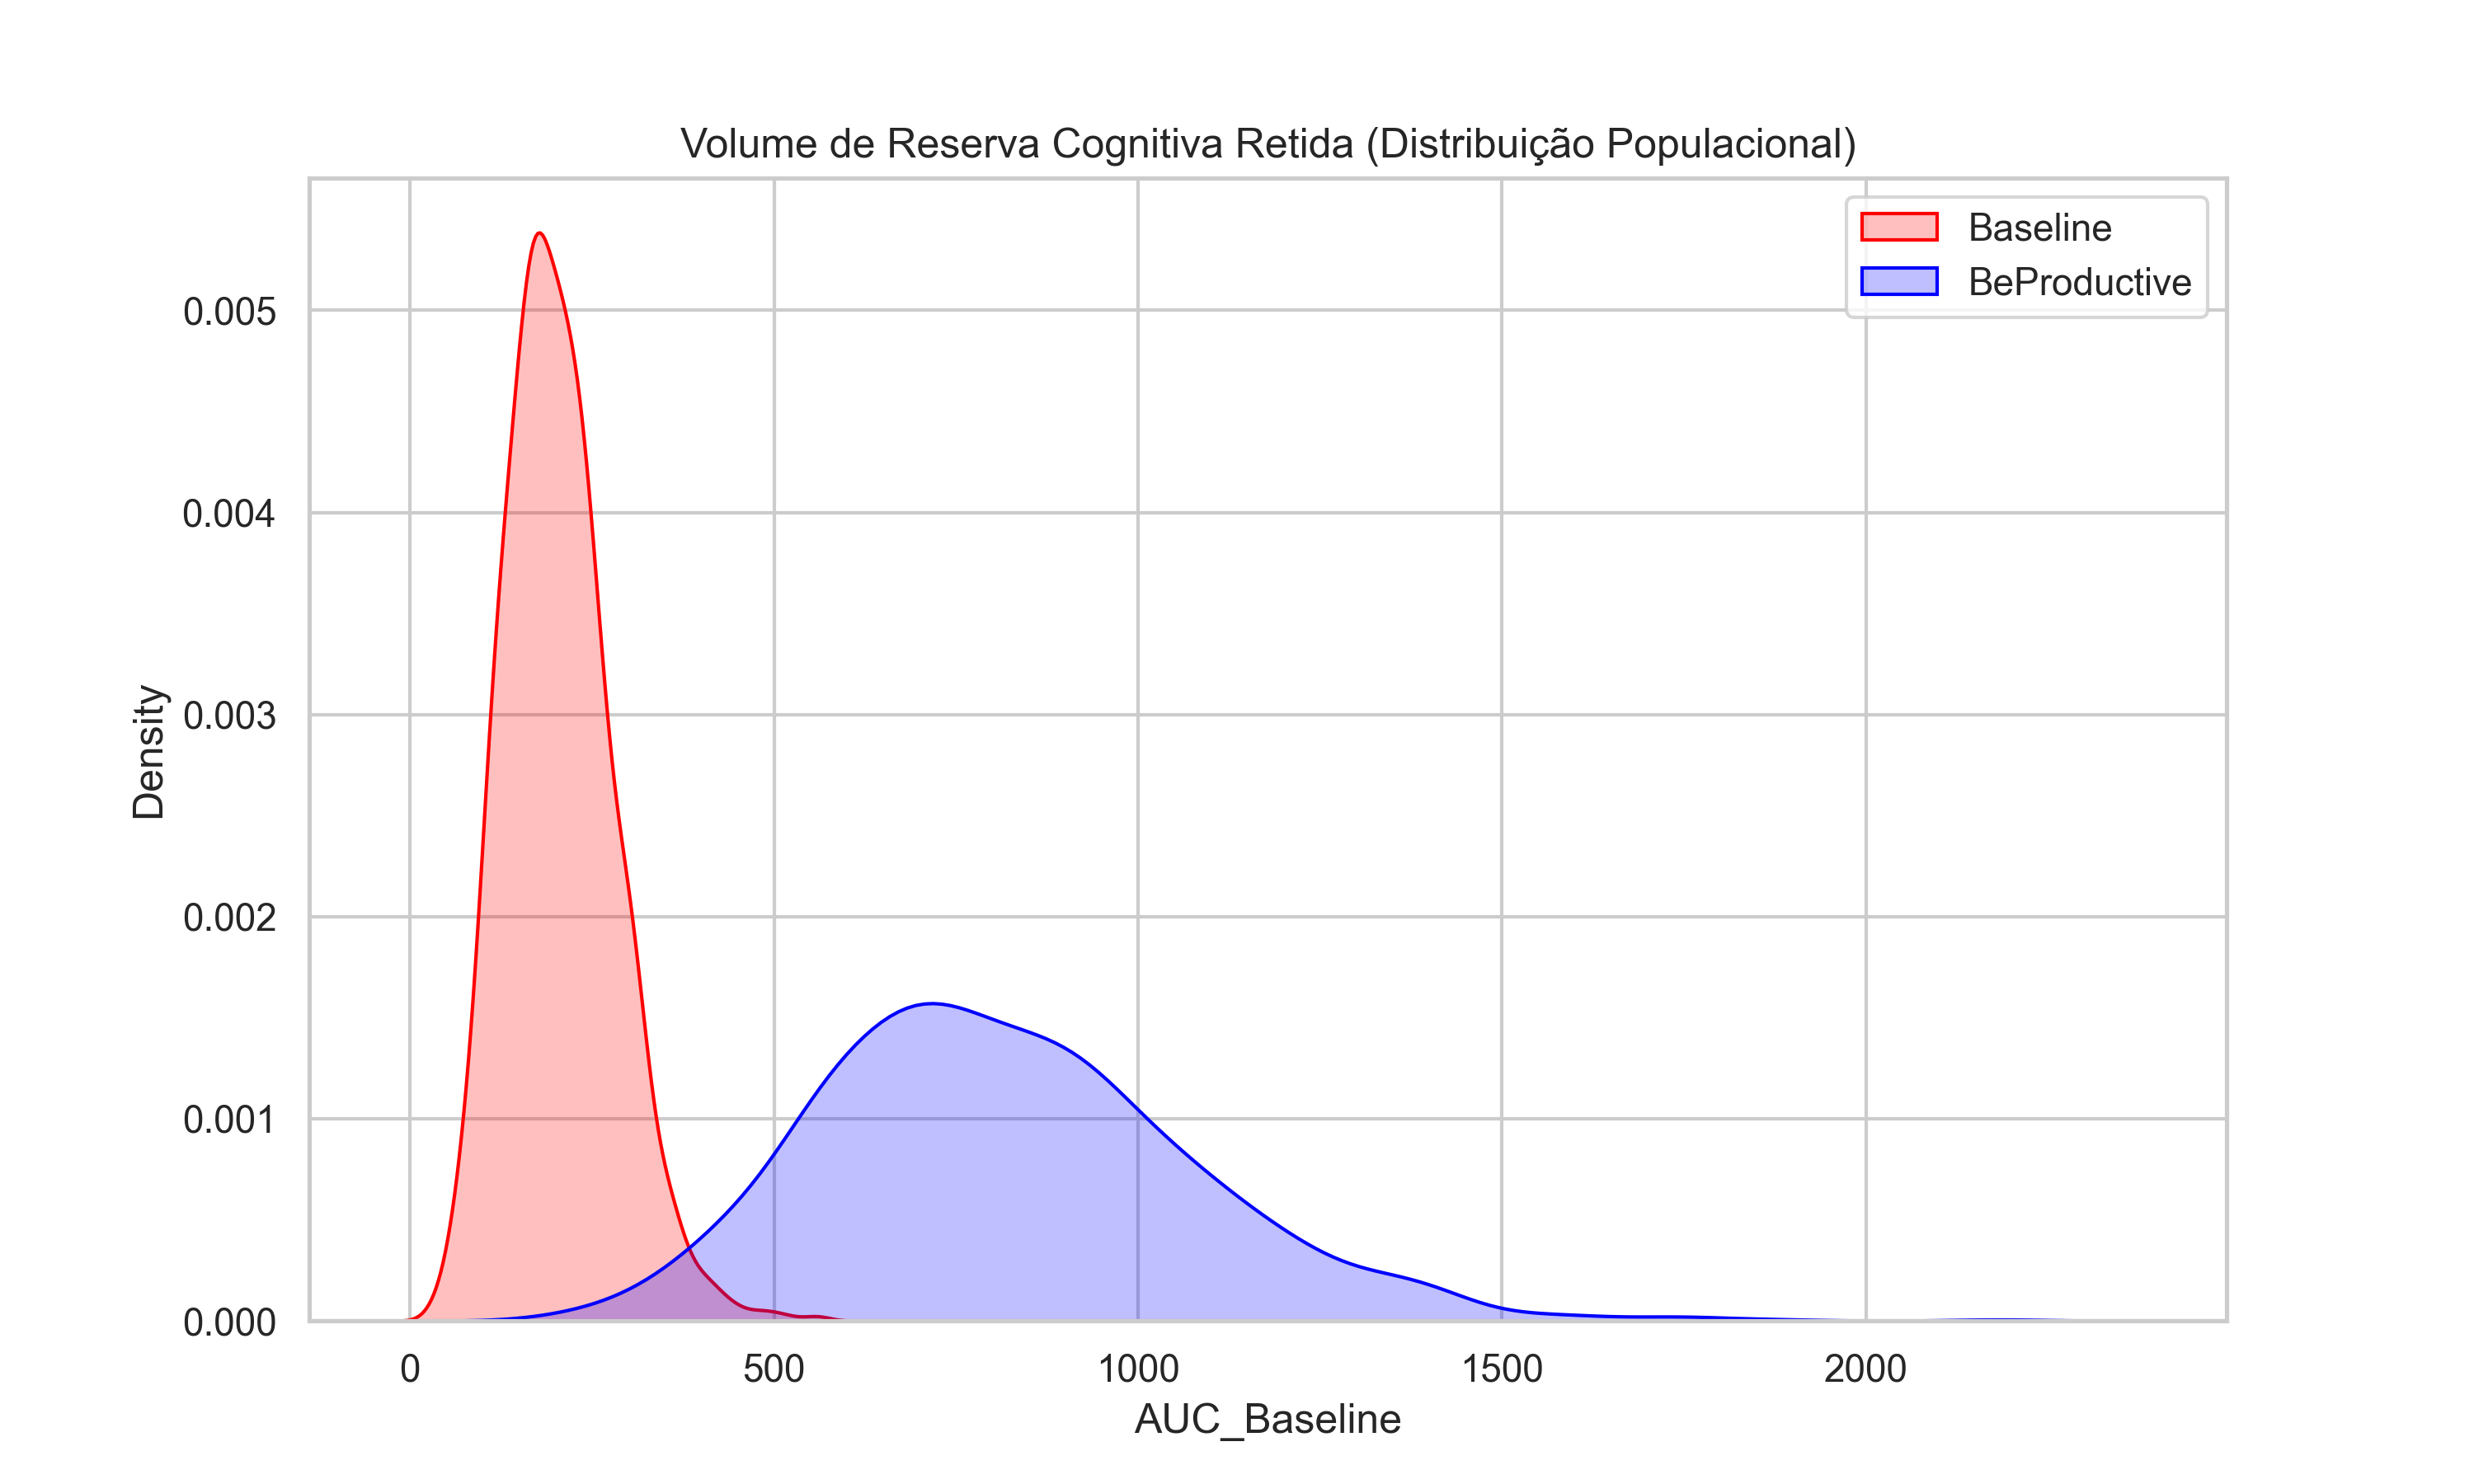
\includegraphics[width=\columnwidth]{../../fig_1_ego_depletion.png}
\caption{Estimativa de Densidade de Kernel (KDE) da {\'A}rea Sob a Curva de Satura{\c c}{\~a}o Cognitiva em modelo ABM com $N=1000$.}
\label{fig:kde_abm}
\end{center}
\end{figure}

\subsection{Entropia de Inten{\c c}{\~a}o e Diverg{\^e}ncia KL}
Visando o grau de tangibilidade na orienta{\c c}{\~a}o atrelada, quantificamos a efici{\^e}ncia estruturada observada pelos desvios l{\'o}gicos. Aplica{\c c}{\~o}es das an{\'a}lises m{\'e}tricas demonstraram o alocamento das aten{\c c}{\~o}es em alinhamento de Diverg{\^e}ncia KL para aferir o deslocamento atencional em decorr{\^e}ncia algor{\'\i}tmica de predi{\c c}{\~o}es comportamentais da restri{\c c}{\~a}o em interface.

\begin{figure}[htbp]
\begin{center}
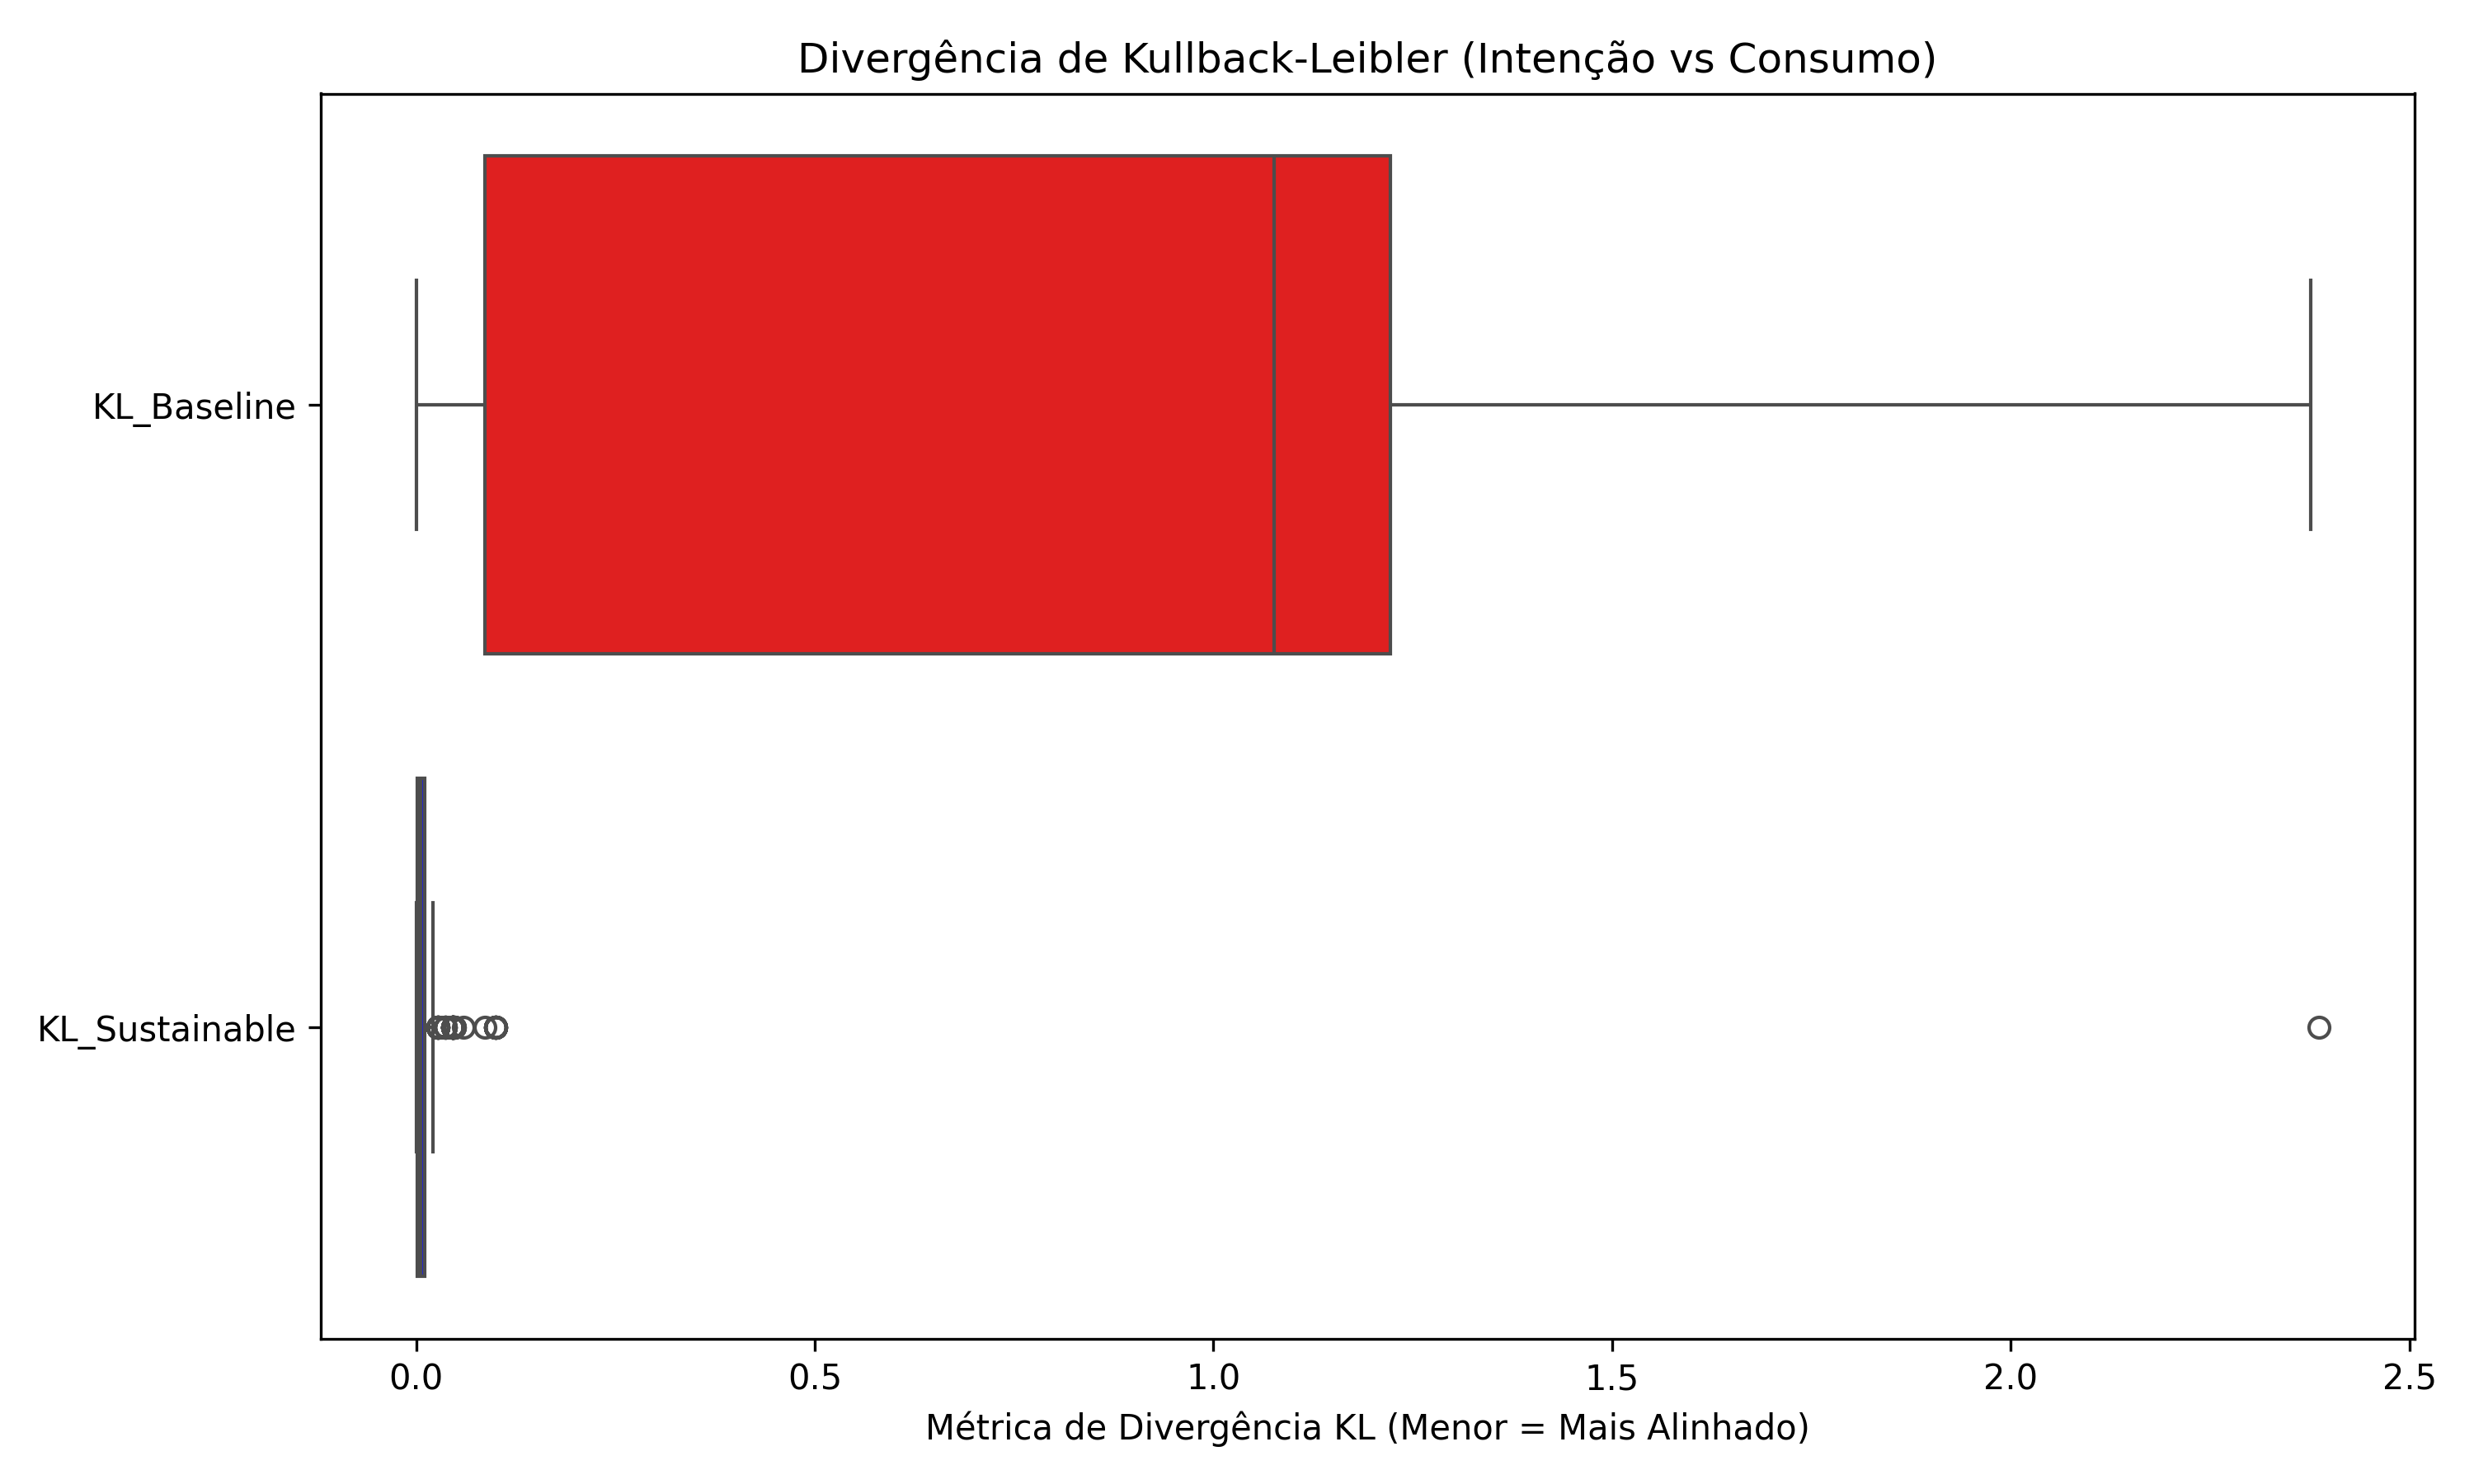
\includegraphics[width=\columnwidth]{../../fig_2_kl_divergence.png}
\caption{Dispers{\~a}o da Diverg{\^e}ncia KL entre inten{\c c}{\~a}o e tempo alocado real.}
\label{fig:kl_boxplot}
\end{center}
\end{figure}

\subsection{Sensibilidade e Testes Monte Carlo}
Redes de testes extensos n{\~a}o-param{\'e}tricos Wilcoxon Rank-Sum endossam as amostras em converg{\^e}ncias e atritam coeficientes restritivos e decaimentos no acompanhamento dos tensores t{\'e}rmicos estipulados para a prote{\c c}{\~a}o ativa sob itera{\c c}{\~o}es rand{\^o}micas. A estabilidade confirmou-se imut{\'a}vel e coerentemente preservada em todo escopo param{\'e}trico vi{\'a}vel na gera{\c c}{\~a}o em teste de atrito com a matriz simulativa t{\'e}rmica.

\begin{figure}[htbp]
\begin{center}
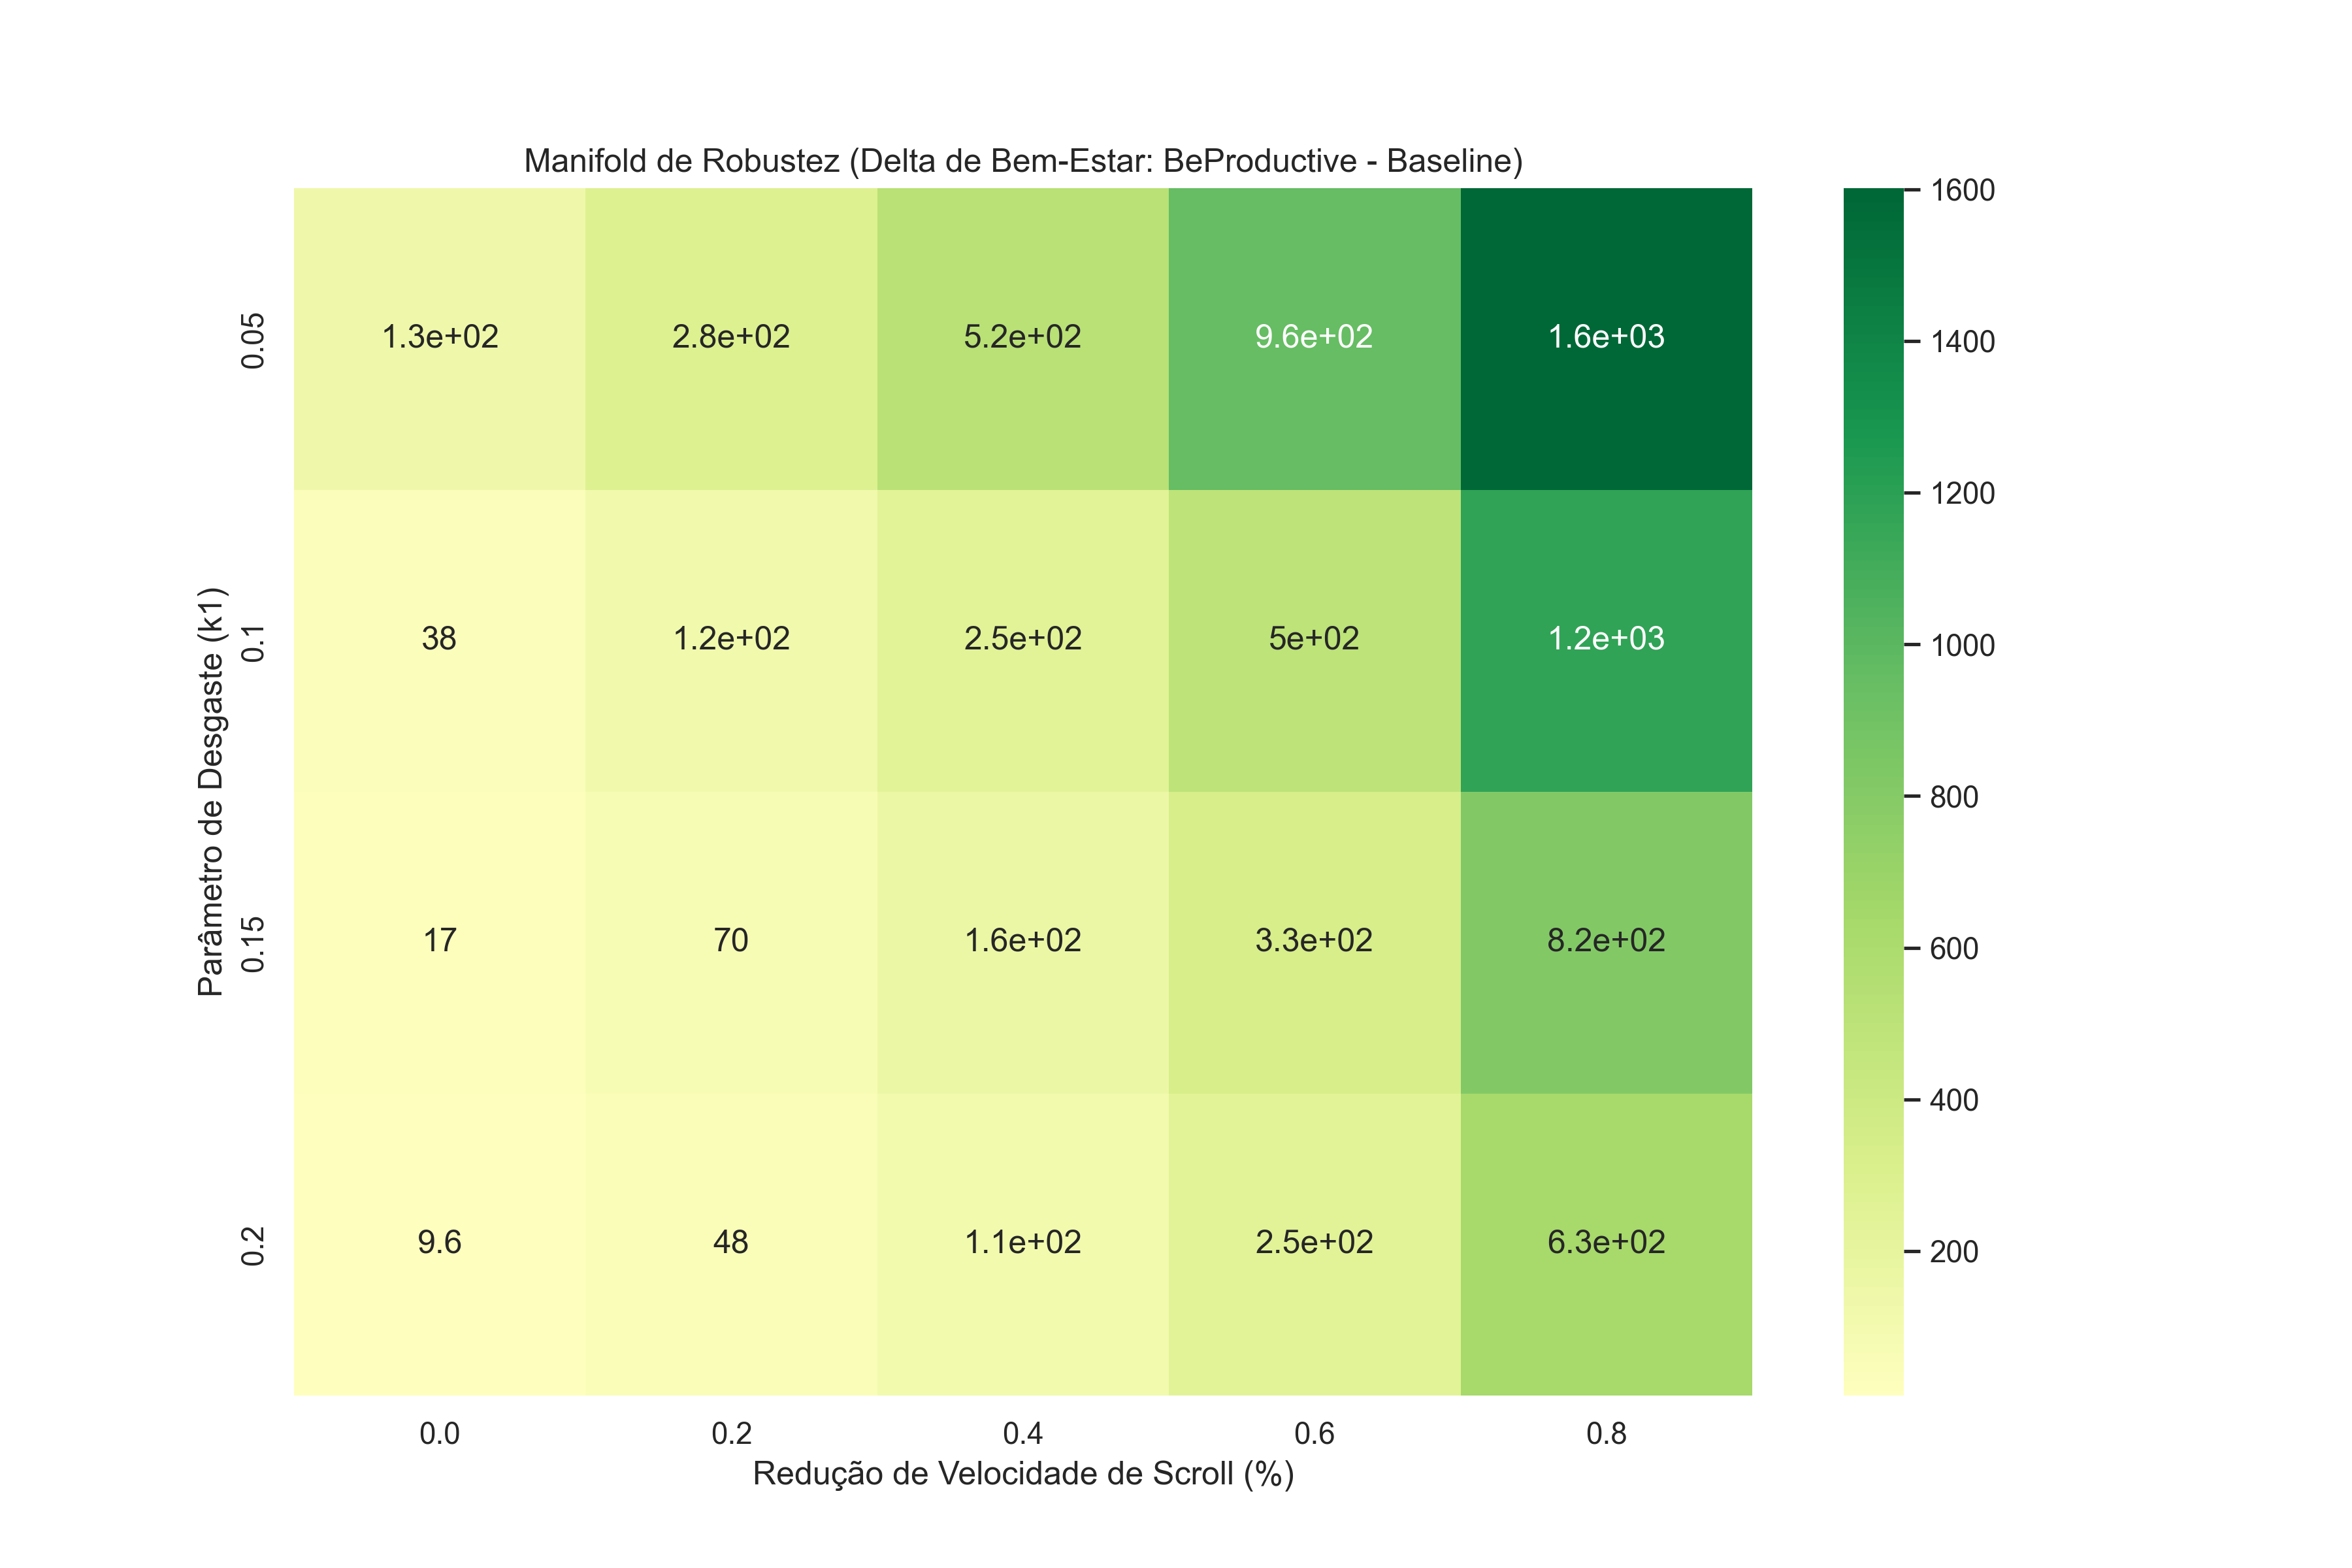
\includegraphics[width=\columnwidth]{../../fig_3_robustness_manifold.png}
\caption{An{\'a}lise de Sensibilidade Monte Carlo da Robustez Atencional.}
\label{fig:monte_carlo}
\end{center}
\end{figure}

\section{Discuss{\~a}o} \label{sec:discussion}

\subsection{Implica{\c c}{\~o}es para Design de RecSys}
A modelagem do \textit{BeProductive} aponta contundentemente que o delineamento de utilidade estrutural cognitiva nos algoritmos preditivos permite convergir alvos de alinhamento restrito (\textit{Value-Aligned}) com elevada efici{\^e}ncia paralela. A incorpora{\c c}{\~a}o do filtro final \textit{min-norm} de probabilidade generativa acoplado por Processos Estoc{\'a}sticos transborda perfeitamente as demandas para al{\'e}m do engajamento simpl{\'o}rio imediato ditado classicamente \citep{carvalho2023, stray2021}. Em um panorama estritamente voltado {\`a} engenharia, provou-se ser inteiramente fact{\'\i}vel alocar sub-rotinas restritivas sob a infer{\^e}ncia em \textit{Edge AI} delegando c{\'a}lculos custosos diretamente aos \textit{endpoints} f{\'\i}sicos de acesso das ferramentas.

\subsection{Considera{\c c}{\~o}es {\'E}ticas Ampliadas}
Essas intera{\c c}{\~o}es n{\~a}o buscam eximir instintivamente os la{\c c}os estritamente funcionais atrelados {\`a}s interrup{\c c}{\~o}es e ao capitalismo de vigil{\^a}ncia por desordem mercen{\'a}ria e compuls{\'o}ria \citep{zuboff2019, citton2017}. Ao predefinir de modo incisivo fun{\c c}{\~o}es normativas por \textit{nudge} condicionado na delega{\c c}{\~a}o consciente pr{\'e}-ativada (\textit{opt-in}), a abordagem atende com fluidez e obviedade aos ditames sociot{\'e}cnicos recomendados por diretrizes da preserva{\c c}{\~a}o tecnol{\'o}gica perante a invas{\~a}o de intimidade atencional sist{\^e}mica e massificada contempor{\^a}nea \citep{cht2026}.

\subsection{Limita{\c c}{\~o}es do Estudo}
Assinalam-se as restri{\c c}{\~o}es inatas ao emprego da simula{\c c}{\~a}o parametrizada (ABM). As disposi{\c c}{\~o}es comportamentais em interrup{\c c}{\~a}o cl{\'\i}nica do racioc{\'\i}nio basearam-se nas infer{\^e}ncias algor{\'\i}tmicas que podem abster componentes ex{\'o}genos inerentes a diferentes dom{\'\i}nios estoc{\'a}sticos emp{\'\i}ricos in-vivo em redes org{\^a}nicas aut{\^e}nticas ao longo do delineamento social ou sob vi{\'e}s param{\'e}trico populacional isolado org{\^a}nico, passivo {\`a}s m{\'e}tricas documentadas no contexto cognitivo real e suas adapta{\c c}{\~o}es flex{\'\i}veis \citep{lyngs2019, kushlev2022}.

\subsection{Agenda de Pesquisa Futura}
Demandas adicionais prospectivas devem almejar averigua{\c c}{\~o}es longitudinais de interrup{\c c}{\~a}o e atrito em testes controlados reais (em formato de testes A/B integrados em aplica{\c c}{\~o}es de larga escala). Futuros ensaios focar{\~a}o estritamente no avan{\c c}o estat{\'\i}stico na mensura{\c c}{\~a}o prolongada da mitiga{\c c}{\~a}o ansiol{\'\i}tica estruturante contra o excesso predat{\'o}rio cognitivo infanto-juvenil documentados, amparando os pain{\'e}is interativos governamentais em regramentos de arquiteturas unificadas em propostas atencionais cl{\'\i}nicas intersecionais psiqui{\'a}tricas padronizadas \citep{brasil_sd, hai2021, costello2023}.

\section{Conclus{\~a}o} \label{sec:conclusion}

O avan{\c c}o sustent{\'a}vel no desenvolvimento dos espa{\c c}os informacionais depende de reformula{\c c}{\~o}es e balan{\c c}os interativos que encerrem efetivamente o desgaste e colapso massivo do foco por arranjos extrativistas passivos contempor{\^a}neos. A presente pesquisa instanciou e quantificou a viabilidade arquitet{\^o}nica para as plataformas priorizarem o foco ativo sem prescindir a viabilidade matem{\'a}tica t{\'e}cnica anal{\'\i}tica que prov{\^e} as bases da l{\'o}gica estruturadora de controle.

As quatro frentes modeladas englobam sistematicamente: (1) o condicionamento por interm{\'e}dio dos Processos de Hawkes que segregam os saltos da estocasticidade baseada pelo engajamento vol{\'a}til transit{\'o}rio dos v{\'\i}nculos de interesse profundo de Sistema 2; (2) a ado{\c c}{\~a}o ativa do desgaste de Equa{\c c}{\~o}es Diferenciais Ordin{\'a}rias (EDO) como restri{\c c}{\~a}o cinem{\'a}tica atencional; (3) a conformidade incontestavelmente resoluta no isolamento \textit{on-device} da arquitetura \textit{Edge AI} garantindo a normatiza{\c c}{\~a}o estrutural inata de conformidade t{\'e}cnica pela privacidade \textit{by design}; e (4) as travas algor{\'\i}tmicas l{\'o}gicas contra fatores temporais do vi{\'e}s do desconto hiperb{\'o}lico.

Evid{\^e}ncias fundamentadas por via dos tensores sint{\'e}ticos em coortes interativas (1.000 inst{\^a}ncias virtuais em simula{\c c}{\~a}o ABM) revelaram robusta consist{\^e}ncia ($d = 3.25$) na conten{\c c}{\~a}o estrutural, atenuando a entropia entre execução observada e interesse humano natural (significância em $p < 10^{-300}$). As soluções tecnológicas atestam não somente factibilidade computacional em rebalanceamento funcional ético, mas também pragmatismo frente aos paradigmas essenciais da inovação contemporânea da Interação Humano-Computador.

\section*{Declarations}

\begin{contributions}
FM contributed to the conception and design of this study, the mathematical modelling, the implementation of the system architecture, and the agent-based simulation. FM is the main contributor and writer of this manuscript.
\end{contributions}

\begin{interests}
The authors declare that they have no competing interests.
\end{interests}

\begin{acknowledgements}
This work was developed as part of an academic project at UNIG (Centro Universitário de Itaguaí).
\end{acknowledgements}

\begin{funding}
This research received no specific grant from any funding agency in the public, commercial, or not-for-profit sectors.
\end{funding}

\begin{materials}
The datasets and softwares generated and analysed during the current study are available in the project repository.
\end{materials}

\bibliographystyle{apalike-sol}
\bibliography{referencias}

\end{document}
